\documentclass{article}

\usepackage{fancyhdr}
\usepackage{cmap}
\usepackage[T2A]{fontenc}
\usepackage[utf8]{inputenc}
\usepackage[english,russian,ukrainian]{babel}
\usepackage{pythontex}
\usepackage{indentfirst}
\usepackage{graphicx}
\usepackage{multirow}
\usepackage{hyperref}
\hypersetup{
	colorlinks,
	citecolor=black,
	linkcolor=black,
	filecolor=black,
	urlcolor=black
}

\usepackage{geometry}
\geometry{
	a4paper,
	total={155mm,247mm},
	left=30mm,
	top=30mm,
}

\usepackage{listings}
\usepackage{xcolor}

\definecolor{codegreen}{rgb}{0,0.6,0}
\definecolor{codegray}{rgb}{0.5,0.5,0.5}
\definecolor{codepurple}{rgb}{0.58,0,0.82}
\definecolor{backcolour}{rgb}{0.99,0.99,0.99}
\definecolor{codeblue}{rgb}{0.1,0.1,0.99}

\lstdefinestyle{mystyle}{
	backgroundcolor=\color{backcolour},   
	commentstyle=\color{codegreen},
	keywordstyle=\color{codeblue},
	numberstyle=\tiny\color{codegray},
	stringstyle=\color{codepurple},
	basicstyle=\ttfamily\footnotesize,
	breakatwhitespace=false,         
	breaklines=true,                 
	captionpos=b,                    
	keepspaces=true,                 
	numbers=left,                    
	numbersep=5pt,                  
	showspaces=false,                
	showstringspaces=false,
	showtabs=false,                  
	tabsize=4
}

\lstset{style=mystyle}

\pagestyle{fancy}
\fancyhf{}
\renewcommand{\headrulewidth}{0.5pt}
\renewcommand{\footrulewidth}{0.5pt}

\begin{document}
	
	\begin{titlepage}
\centering{
	
\includegraphics[width=\textwidth]{institute.jpg}
	\large 
		\vspace{0cm}\\
		Міністерство освіти і науки України \\
		Національний технічний університет України \\
		"Київський політехнічний інститут імені Ігоря Сікорського"\\
		Фізико-технічний інститут
	}
	\vspace{4cm}\\
	\centering{
		{\Huge	\textbf{Алгоритми та структури даних} \\ \vspace{0.15cm}}
		{\LARGE Лабораторна робота №2}
	}
	
	\vspace{7.5cm}
	\Large
	\begin{flushright}
		Виконав: студент групи ФБ-82\\
		Козачок Вячеслав\\
		Перевірила: \\
		Лавренюк 
	\end{flushright}
	\vfill
	
	\centering{Київ - 2020}
	
\end{titlepage}
	
\Large	
\textbf{Мета:} Познайомитися з роботою поширених методів сортування, з критеріями та методикою їх порівняння. \\

	\textbf{Варіант:} $9 - 6= 3$
	\begin{itemize}
	\item  Сортування методом бульбашки;
	\item Сортування методом Шелла.
	\end{itemize}
\section*{\centering {Хід роботи:}}

\large Не відсортований масив:\\
\texttt{
9384 887 2778 6916 7794 8336 53 9384 887 2778 6916 7794 8336 5387 493 6650 1422 2363 28 869160 7764 3927 541 3427 9173 5737 5212 5369 2568 6430 5783 1531 2863 5124 4068 3136 3930 9803 4023 3059 3070 8168 1394 8457 5012 8043 6230 7374 4422 4920 3785 8538 5199 4325 8316 4371 6414 3527 6092 8981 9957 1874 6863 9171 6997 7282 2306 926 7085 6328 337 6506 847 1730 1314 5858 6125 3896 9583 546 8815 3368 5435 365 4044 3751 1088 6809 7277 7179 5789 3585 5404 2652 2755 2400 9933 5061 9677 3369 7740 13 6227 8587 8095 7540 
}


\large Відсортований масив:\\ 
\texttt{
13 28 60 337 365 493 541 546 847 887 926 1088 1314 1394 1422 1531 1730 1874 2306 2363 2400 2568 2652 2755 2778 2863 3059 3070 3136 3368 3369 3427 3527 3585 3751 3785 3896 3927 3930 4023 4044 4068 4325 4371 4422 4920 5012 5061 5124 5199 5212 5369 5387 5404 5435 5737 5783 5789 5858 6092 6125 6227 6230 6328 6414 6430 6506 6650 6809 6863 6916 6997 7085 7179 7277 7282 7374 7540 7740 7764 7794 8043 8095 8168 8316 8336 8457 8538 8587 8691 8815 8981 9171 9173 9384 9583 9677 9803 9933 9957 
}\\

\hspace{-2cm}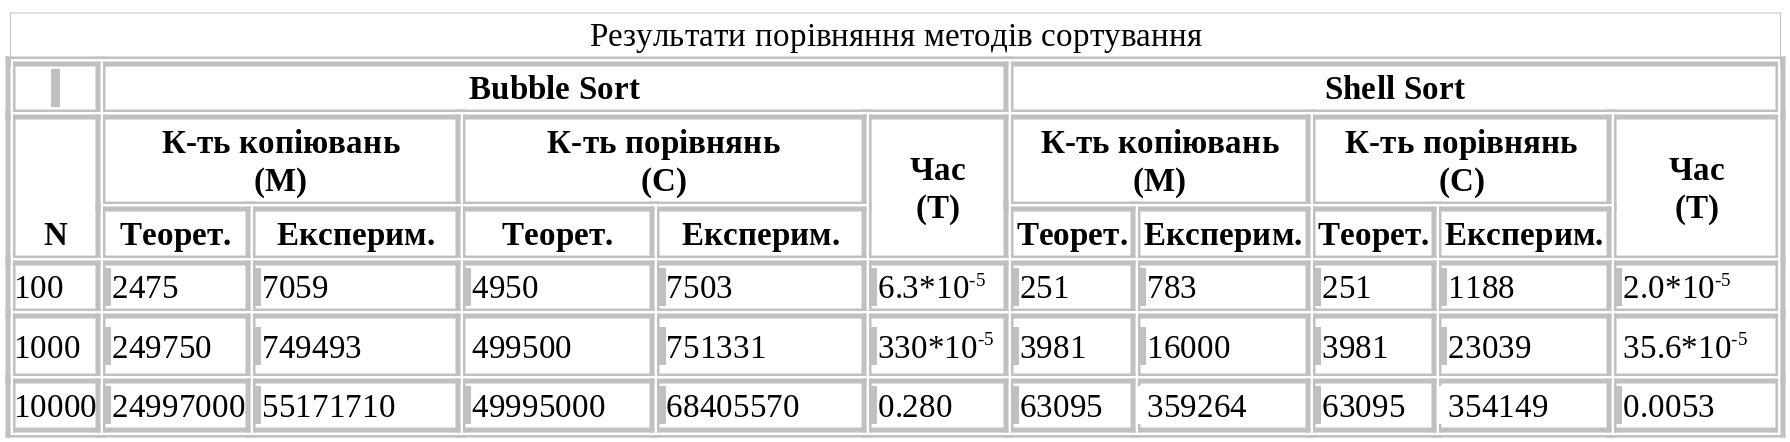
\includegraphics[width=18.5cm]{results.png}

\newpage
\section*{Code}
\begin{lstlisting}[language=C]
#include <iostream>
#include <fstream>
#include <ctime>
#include <cmath>
#include <random>

void printArray(int * a, int n);

void insertionSort(int * arr, int n)  
{  
	int i, key, j;  
	for (i = 1; i < n; i++) 
	{  
		key = arr[i];  
		j = i - 1;  
		
		while (j >= 0 && arr[j] > key) 
		{  
			arr[j + 1] = arr[j];  
			j = j - 1;  
		}  
		arr[j + 1] = key;  
	}  
}  

void bubbleSort(int * arr, int n)
{
	int compare = 0, move = 0;
	for(int i = 0; i < n; i++)
	{
		compare++;
		for(int k = i; k < n; k++)
		{
			compare++;
			if(arr[i] > arr[k])
			{
				compare++;
				int num = arr[i];
				arr[i] = arr[k];
				arr[k] = num;
				move += 3;
			}
		}
	}
	std::cout << "Compares: " << compare << ", Moves: " << move << std::endl;
	
}


void shellSort(int * arr, int n)
{
	
	
	int stepsNum = (int)log2(n) - 1 ;
	int * steps = new int[stepsNum];
	steps[stepsNum-1] = 1;
	
	for(int i = stepsNum-2;i >= 0; i--)
	steps[i] = 2 * steps[i+1] + 1;
	
	std::cout << stepsNum << "; ";
	printArray(steps, stepsNum);
	
	
	int i, j, increment, temp;
	int move = 0, compare = 0;
	
	// for(increment = n/2; increment > 0; increment/=2)
	for(int k = 0; k < stepsNum; k++ )
	{   
		compare++;
		move++;
		increment = steps[k];
		for(i = increment; i < n; i++)
		{
			compare++;
			temp = arr[i];
			for(j = i; j >= increment ;j-=increment)
			{
				//perform the insertion sort for this section
				compare++;
				if(temp < arr[j-increment])
				{
					move++;
					arr[j] = arr[j-increment];
				}
				else
				{
					break;
				}
			}
			move++;
			arr[j] = temp;
		}
	}
	std::cout << "Compares: " << compare << ", Moves: " << move << std::endl;
	
}

void printArray(int * a, int n)
{
	for(int i = 0; i < n; i++)
	{
		std::cout << a[i] << ' '; 
	}
	std::cout << std::endl;
}

int *  fillArray(int n)
{
	int * arr = new int[n];
	for(int i = 0; i < n; i++)
	{
		arr[i] = rand() % 10000 + 1;
	} 
	return arr;
}


void call(void (&func)(int* arr , int n), int * arr, int n)
{
	clock_t t = clock();
	(*func)(arr, n);
	std::cout << "Sort time: " << ((double)(clock() - t))/CLOCKS_PER_SEC << std::endl;
}

int main(int argv, char** argc) {
	
	int n = 100;
	int * arr = fillArray(n);
	std::cout << "1. Bubble Sort\n2. Shell Sort" << std::endl;
	int choice;
	
	std::cin >> choice;
	
	printArray(arr, n);
	if(choice == 1) call(bubbleSort, arr, n);
	if(choice == 2) call(shellSort, arr, n);
	printArray(arr, n);
	
	return 0;
}
\end{lstlisting}

\newpage
\section*{Висновки}
Під часвиконання роботи, я вивчив такі алгоритми сортування як \texttt{Shell Sort}, \texttt{Insertion Sort} та \texttt{Bubble Sort}.
Навчився заміряти час роботи алгоритмів, робити теоретичну оцінку їх швидкодії.
Навчився передавати функцію, як аргумент у іншу функцію.


\end{document}
